\section{Narzędzia użyte podczas pisania pracy} \label{narzedzia}

Realizując założenia pracy inżynierskiej użyto podczas jej tworzenia całej gamy narzędzi. Proces tworzenia przebiegał w~systemie operacyjnym GNU~Linux \cite{kernel} (dystrybucja Ubuntu \cite{ubuntu}).

\subsection{Kontrola pracy w~Scrum}

Narzędzia użyte do kontroli przebiegu pracy nad projektem zostały opisane poniżej.

\subsubsection{Git}

\textit{Git} \cite{git} to~rozproszony system kontroli wersji. Stworzył go~Linus Torvalds jako narzędzie wspomagające rozwój jądra Linux. \textit{Git} stanowi wolne oprogramowanie i~został opublikowany na~licencji GNU~GPL w~wersji~2.

Pierwsza wersja narzędzia \textit{Git} została wydana 7~kwietnia~2005 roku, by~zastąpić poprzednio używany w~rozwoju systemu Linux, niebędący wolnym oprogramowaniem, system kontroli wersji \textit{BitKeeper}.


Wiele projektów używa \textit{Git} jako systemu kontroli wersji, zarówno nowo powstające, jak i~migrujące do~niego z~innego systemu kontroli wersji (na~przykład~z~CVS lub SVN). Do~największych i~najbardziej znanych projektów o~otwartym źródle, należy wymienić: jądro Linuksa oraz~podprojekty z~nim związane, a~także GNU~Hurd, GNOME, GTK+, GStreamer, KDE, GIMP, Perl, Qt, Ruby~on~Rails, Samba, Wine, Xfce, Xorg, jQuery, YUI, Erlang. Również część serwisów internetowych używa \textit{Git} do~rozwijania swojego kodu (a~część z~niego jest publicznie dostępna), m.in.~\textit{Reddit} (otwarte źródła), \textit{Digg}, czy \textit{Facebook}.


Kilka systemów operacyjnych korzysta z~\textit{Git} do~zarządzania całą dystrybucją oraz~dodatkowymi programami w~nie wchodzącymi: Arch Linux, Android, Fedora, Maemo, MeeGo, OLPC~XO-1, openSUSE oraz DragonFly~BSD. Dystrybucje Debian oraz~Ubuntu używają \textit{Git} do~rozwijania programów oraz~zmian w~programach zewnętrznych dla wielu (choć nie wszystkich) pakietów.

\subsubsection{tig}

\texttt{tig} (Rys. \ref{tool.tig}) to~narzędzie \texttt{ncurses} służące do~prostego zarządzania repozytorium \texttt{git}. Jest dobrą alternatywą dla wbudowanego w~pakiet narzędzi systemu Git \texttt{gitg}, pozwalającą na~wykorzystanie identycznych funkcjonalności w~konsoli.

\subsubsection{ticgit}

\texttt{ticgit} \cite{ticgit} (Rys. \ref{tool.ticgit}) to~prosty \textit{issue tracker} (narzędzie do~zarządzania zadaniami, związanymi z~projektem) działający jako rozszerzenie dla systemu kontroli wersji \textit{Git}. Zapisuje zmiany w~trackingu w~oddzielnej gałęzi repozytorium \textit{Git} projektu. Pozwala to~na~przechowywanie dokumentacji dotyczącej rozwoju projektu wraz z~kodami źródłowymi.

\begin{figure}[ht]
\centering
\fbox{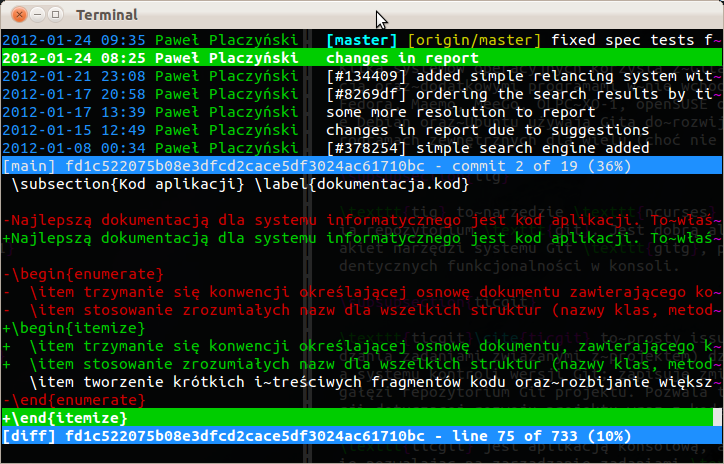
\includegraphics[width=\textwidth]{obrazki/tig.png}}
\caption{Program \textit{tig} podczas pracy nad repozytorium projektu.}
\label{tool.tig}
\end{figure}

\texttt{ticgit} jest aplikacją konsolową, aczkolwiek istnieje rozszerzenie pozwalając na~zarządzanie zadaniami \texttt{ticgit} przy pomocy przeglądarki internetowej i~prostego interfejsu webowego \cite{ticgitweb}.

\begin{figure}[ht]
\centering
\fbox{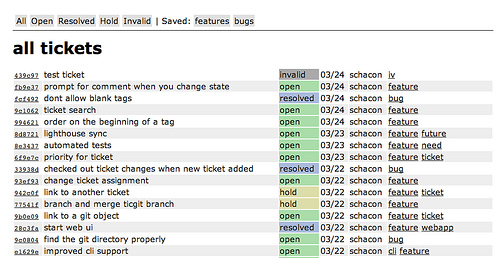
\includegraphics[width=\textwidth]{obrazki/ticgitweb.png}}
\caption{Webowy interfejs \textit{ticgitweb} dla narzędzia zarządzania zadaniami \textit{ticgit}}
\label{tool.ticgit}
\end{figure}

\subsection{Środowisko programistyczne}

Oprócz systemu operacyjnego potrzebne są także narzędzia do zarządzania środowiskiem programistycznym (język programowania, bibilioteki, wtyczki), a także narzędzia wspomagające programowanie jak edytory tekstu, konsole).

\subsubsection{zsh + GNU~Screen}

Większość pracy nad projektem napisanym przy pomocy frameworku Ruby~on~Rails odbywa się w~konsoli. Jako powłoki użyto powłoki \textit{Open-Source} \texttt{zsh} \cite{zsh}. Powłoka ta~udostępnia rozbudowany i~przyjazny użytkownikowi system podpowiedzi (system ten zintegrowany jest z~wieloma poleceniami konsoli, w~tym z~narzędziami systemu kontroli wersji \textit{Git}), jak również udogodnienia dotyczące historii wykonywanych poleceń, autokorektę oraz~szereg opcji konfiguracji zachowania i~wyglądu.


\texttt{screen} \cite{screen} jest narzędziem pozwalającym na~sprawne zarządzanie uruchomionymi powłokami/poleceniami. Pozwala~na:

\begin{itemize}
  \item przełączanie się pomiędzy uruchomionymi powłokami/poleceniami,
  \item pracę w~kilku oknach (widokach),
  \item odłączanie się (\textit{deteach}) i~pozwalanie na kontynuację wykonywanych poleceń (opcja przydatna podczas pracy zdalnej),
  \item kopiowanie/wklejanie/przeszukiwanie ekranu konsoli,
  \item wyświetlanie informacji o~systemie/procesach w~dolnej linijce ekranu.
\end{itemize}

\subsubsection{Vim}

\textit{Vim} \cite{vim} (Rys. \ref{tool.vim}) według oficjalnej interpretacji oznacza \texttt{vi improved}. Jest to~wieloplatformowy klon edytora tekstu \texttt{vi}, napisany przez Brama Moolenaara, holenderskiego programistę.

\begin{figure}[ht]
\centering
\fbox{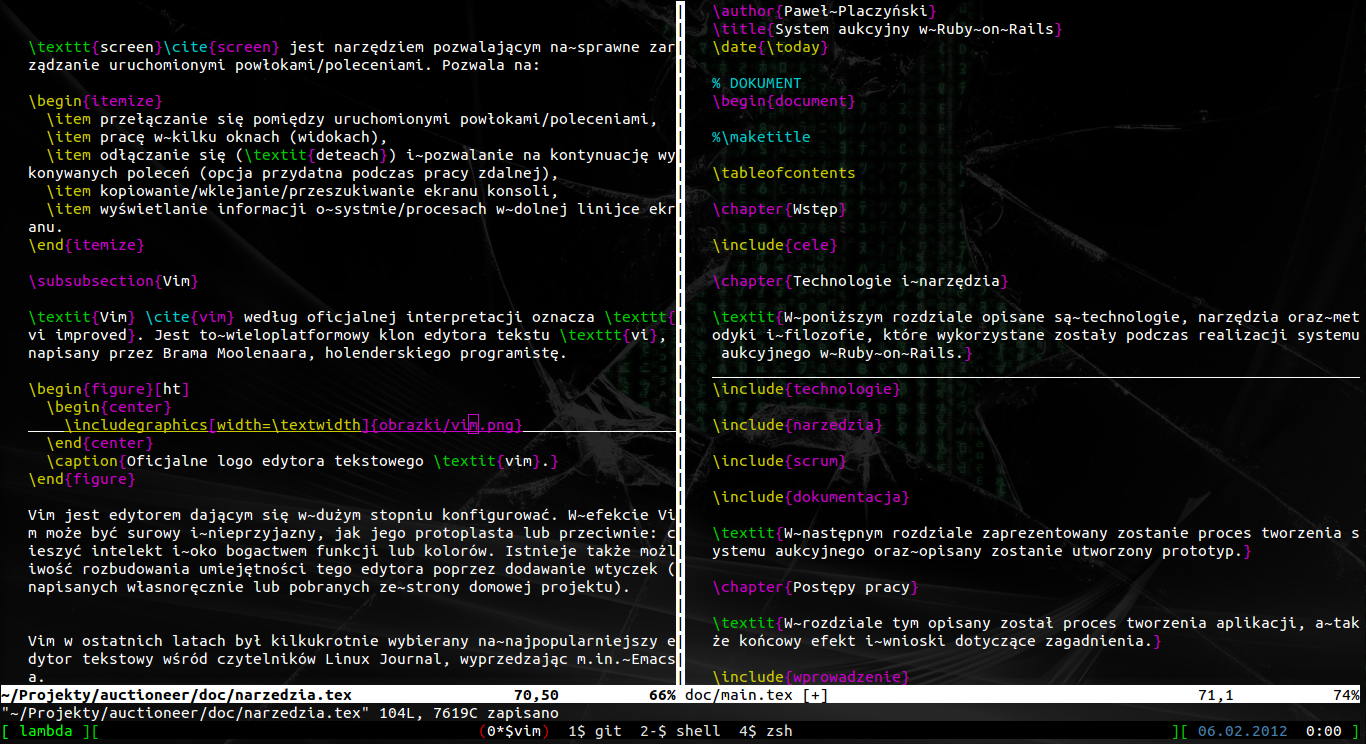
\includegraphics[width=\textwidth]{obrazki/vim.png}}
\caption{Program \textit{Vim} podczas pracy}
\label{tool.vim}
\end{figure}

\textit{Vim} jest edytorem dającym się w~dużym stopniu konfigurować. W~efekcie \textit{Vim} może być surowy i~nieprzyjazny, jak jego protoplasta lub przeciwnie: cieszyć intelekt i~oko bogactwem funkcji lub kolorów. Istnieje także możliwość rozbudowania umiejętności tego edytora poprzez dodawanie wtyczek (napisanych własnoręcznie lub pobranych ze~strony domowej projektu).


\textit{Vim} w~ostatnich latach był kilkukrotnie wybierany na~najpopularniejszy edytor tekstowy wśród czytelników Linux Journal, wyprzedzając m.in.~\textit{Emacs}.

\subsubsection{RVM}

\textit{RVM} \cite{rvm} to~system kontroli wersji języka Ruby. Pozwala na~zainstalowanie wielu implementacji i~wersji tego języka na~lokalnej maszynie oraz~proste zarządzanie wtyczkami \texttt{Gem} dla tych implementacji. Umożliwia proste przełączanie się pomiędzy wersjami języka.

\subsubsection{IRB}

\textit{IRB} to~interaktywna konsola języka Ruby udostępniana wraz z~tym językiem. Jest podobna w~działaniu do~konsoli języka Python, a~zatem udostępnia szereg opcji, pozwalających na~testowanie małych porcji kodu jezyka Ruby w~,,biegu''. Możliwe jest także skonfigurowanie zachowań konsoli IRB przy pomocy skryptów napisancych w~języku Ruby (na~przykład~kolorowanie składni, formatowanie wyjścia konsoli).

\subsubsection{Sqliteman}

\textit{Sqliteman} \cite{sqliteman} to~narzędzie do~zarządzania bazami danych \textit{Sqlite3}. Oferuje graficzny interfejs, pozwalający na~szybkie przeglądanie/edycję zawartości bazy danych.

\subsection{Wdrożenie}

Do~pełnego przedstawienia cyklu pracy nad projektem wykonanym w~technologii Ruby~on~Rails potrzebne jest przedstawienie metod wdrożenia aplikacji webowej oraz~zaproponowanie sposobu jej konserwacji. W~tym celu przybliżono jedno z~najprostszych sposobów wdrożenia aplikacji Ruby~on~Rails.

\subsubsection{Heroku}

\textit{Heroku} \cite{heroku} to~serwis pozwalający na~uruchamianie i~konserwację projektów napisanych w~języku Ruby ,,w~chmurze''.


\textit{Heroku} wykorzystuje \textit{cloud-computing} do~wdrażania alpikacji webowych, opartych na~interfejsie \textit{Ruby~Rack} (aplikacji Ruby~on~Rails, Sinatra, itp.). Pozwala to~na~odrzucenie zbędnego planowania oraz~konfiguracji/konserwacji środowisk uruchomieniowych. Zmniejsza to~koszt zatrudnienia administratorów, a~także koszt sprzętu lub niezbędnych usług (połączenie internetowe, certyfikaty, domeny).


\textit{Heroku} nie jest jedyną taką usługą dostępną dla programistów Ruby, jednakże tylko ono~pozwala na~założenie niewielkich aplikacji testowych.
